\documentclass[a4paper]{article}
\usepackage{graphicx}
\usepackage[hidelinks]{hyperref}
\usepackage[labelformat=empty]{subcaption}
\usepackage{amsmath}

\author{
  Bettermann, Patrick
  \and
  Madlener, Christoph
  \and
  Scheller, Lisa
}

\title{DG Lab Project Report -- Magnetohydrodynamics}

\begin{document}
\maketitle

Lisa implemented the eigenvalues, the Kelvin-Helmholtz instability and
experimented with an alternative divergence cleaning approach. Patrick focused
on the theoretical background and assisted in the flux implementation and
testing. The flux as a whole was a team effort. Christoph implemented the rotor
and Orszag-Tang scenarios, required changes in the infrastructure and cleaned up
the code.

\section{Background and Governing Equations}
The magnetohydrodynamics equations (for brevity referred to as the MHD
equations) are a set of nonlinear hyperbolic partial differential equations used
to describe the movement of an electrically conducting fluid, which is not only
influenced by hydrodynamic processes but also electromagnetic processes. This
means that the fluid has to conform to the already discussed Euler equations,
but also to the Maxwell equations of electrodynamics. An example application for
such a fluid would be solar plasma. There are 8 equations, in the conservative
formulation the varibales are the density $\rho$, the momentum components $\rho
u$, $\rho v$, $\rho w$, the energy $E$ and the magnetic field components $B_x$,
$B_y$, $B_z$.\\
The equations for ideal MHD are as follows \cite{dedner2002hyperbolic}\cite{balsara2010multidimensional}:
\begin{align*}
\delta_t \rho + \bigtriangledown \cdot (\rho\textbf{u})= 0\\
\delta_t (\rho \textbf{u}) + \bigtriangledown \cdot (\rho     \textbf{u} \textbf{u}^T + (p + \dfrac{|\textbf{B}|^2}{8\pi})I - \dfrac{1}{4\pi}\textbf{B}\textbf{B}^T) = 0\\
\delta_t B + \bigtriangledown \cdot (\textbf{uB}^T-\textbf{Bu}^T) = 0\\
\delta_t E + \bigtriangledown \cdot ((E + p + \dfrac{|\textbf{B}|^2}{8\pi})\textbf{u} - \dfrac{1}{4\pi}\textbf{B}(\textbf{u} \cdot \textbf{B})) = 0\\
\end{align*}
where $\textbf{u} = (u, v, w)$ and $\textbf{B} = (B_x, B_y, B_z)$.\\
A split of these equations into partial derivatives into x, y and z direction can also be found in \cite{balsara2010multidimensional}.
The relation between pressure and energy is given by the following equation~\cite{dedner2002hyperbolic}.
\begin{align*}
p = (\gamma - 1)(E - \dfrac{1}{2}\rho |\textbf{u}|^2 - \dfrac{1}{8\pi} |\textbf{B}|^2)
\end{align*}
\subsection{Eigenvalues}
The system of equations has the following eigenvalues for one dimension\cite{dedner2002hyperbolic}:\\
$u$, $u \pm c_s$, $u \pm c_a$ and $u \pm c_f$. \\
Here 
\begin{align*}
c_a &= |b_x|,\\
c_s &= \sqrt{\dfrac{1}{2}(a^2 + b^2 - \sqrt{(a^2 + b^2)^2 - 4a^2b_x^2}))}\\
c_f &= \sqrt{\dfrac{1}{2}(a^2 + b^2 - \sqrt{(a^2 + b^2)^2 - 4a^2b_x^2}))}.\\
\end{align*}
The following abbreviations are used: $b_x = \sqrt{\dfrac{B_x^2}{\rho}}$, $b^2 = \dfrac{|\textbf{B}|^2}{\rho}$ and $a = \sqrt{\dfrac{\gamma p}{\rho}}$.\\
In particular, the highest eigenvalue is $u + c_f$, since $c_f$ is the speed of the fast magnetosonic waves ($c_a$ is the Alfv\'en wave speed and $c_s$ is the slow magnetosonic wave speed).

\section{Divergence Cleaning}
One of the constraints that the Maxwell equations impose on the system is that
the divergence of the magnetic field is zero, thus there are no sources or sinks
of the magnetic field. This constraint can be violated by numerical simulations
because of errors introduced by discretization \cite{dedner2002hyperbolic}.
Furthermore these errors can increase with time. The divergence cleaning scheme
introduced by Dedner \cite{dedner2002hyperbolic} ensures the compliance to this
constraint by coupling the divergence constraint to the conservation laws by a
generalized Lagrange multiplier.

In practice this is done by adding a ninth variable $\Psi$ to the system. This
$\Psi$ is now included in the flux of $\textbf{B}$ by adding $\Psi I$, so the
flux becomes $\textbf{uB}^T-\textbf{Bu}^T + \Psi I$, whereas the flux of $\Psi$
is simply the constant factor $c_h^2$, which can be set to 1 for our
simulations.
\section{Results}
In order to illustrate the obtained results, we chose two well-known examples
for the (ideal) MHD equations.
\subsection{Rotor}\label{sec:rotor}
The first one is the rotor problem~\cite{balsara1999staggered} where an
initially rotating high-density fluid is embedded in a low-density environment
which is at rest. Due to the rapid rotation torsional Alfv\'en waves are launched
into the atmosphere, slowing the rotation down. The magnetic field additionally
compresses the fluid in the rotor into an oblong shape. The simulation was run
on a $500 \times 500$ grid at order 1, see~\autoref{fig:rotor} for a screenshot.
Order 1 was chosen so the limiter could be disabled, as the current
implementation smears the solution heavily. To utilize higher-orders a more
involved limiter (and probably the same holds for the Riemann solver) is required.

\begin{figure}[h]
  \centering
  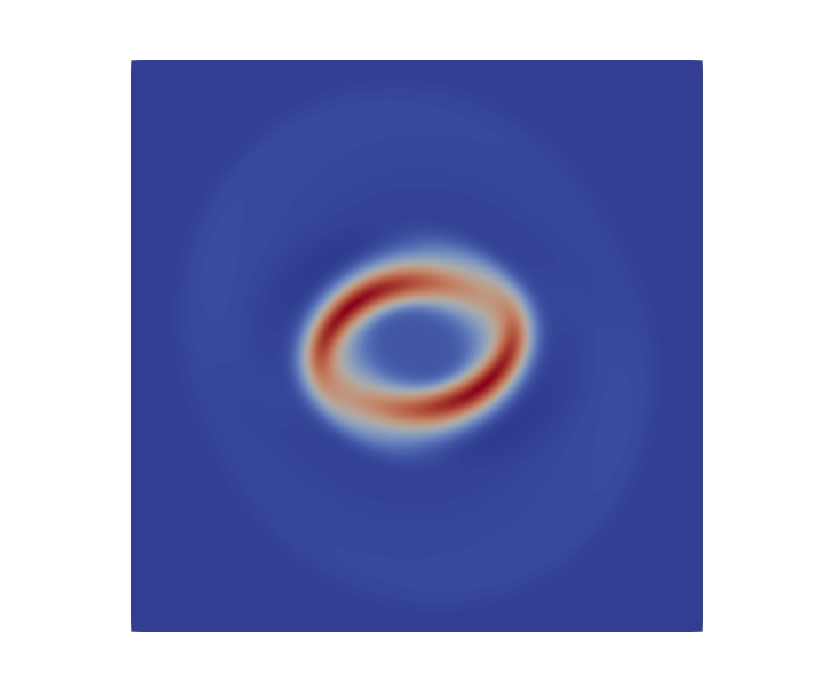
\includegraphics[width=\textwidth]{results/rotor}
  \caption{Density of the rotor problem (\autoref{sec:rotor}) at $t=0.25$. At this point the Alfv\'en
    wave has almost reached the boundary and the rotor is already elongated.}
  \label{fig:rotor}
\end{figure}

\subsection{Orszag-Tang Vortex}\label{sec:orszagtang}
The second example is the also well-known Orszag-Tang vortex, which was first
investigated in relation to singularities arising from MHD
turbulence~\cite{orszag1979small}. We used the initial conditions as given by
Dumbser~\cite{dumbser2019divergence}, which is also a great source for
high-quality figures for both of the presented examples. This simulation was run
on an order 1 grid with $300 \times 300$ elements until $t=5.0$. The results are illustrated
in \autoref{fig:orszagtang}; up until $t=3.0$ the results match the ones
in~\cite{dumbser2019divergence} reasonably well, at $t=5.0$ the smearing of
the Rusanov flux becomes more apparent.

\begin{figure}[h]
  \centering
  \begin{subfigure}[b]{0.49\textwidth}
    \centering
    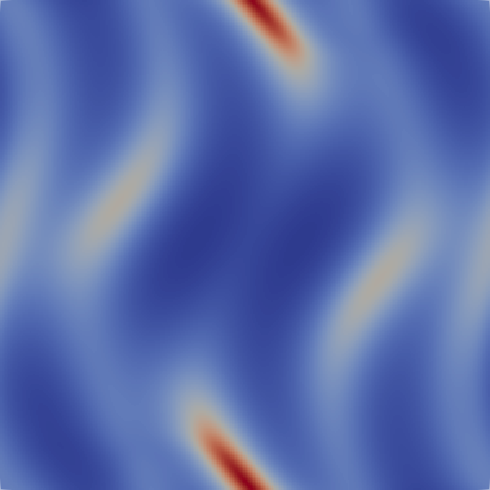
\includegraphics[width=\textwidth]{results/orszag_tang05}
  \end{subfigure}
  \begin{subfigure}[b]{0.49\textwidth}
    \centering
    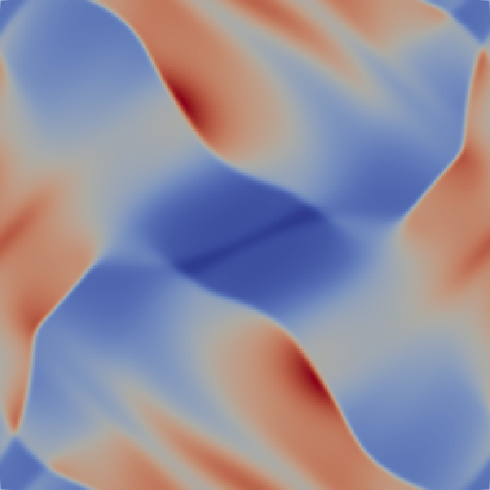
\includegraphics[width=\textwidth]{results/orszag_tang2}
  \end{subfigure}
  \begin{subfigure}[b]{0.49\textwidth}
    \centering
    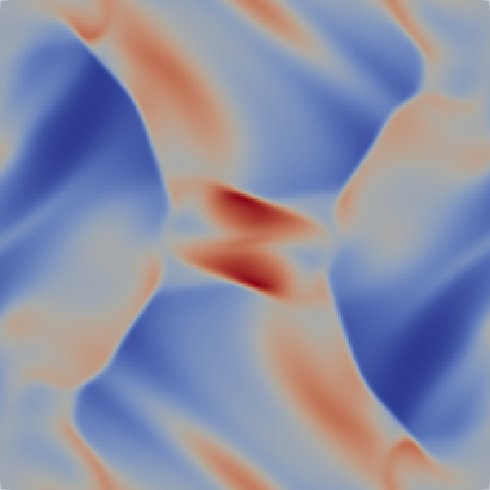
\includegraphics[width=\textwidth]{results/orszag_tang3}
  \end{subfigure}
  \begin{subfigure}[b]{0.49\textwidth}
    \centering
    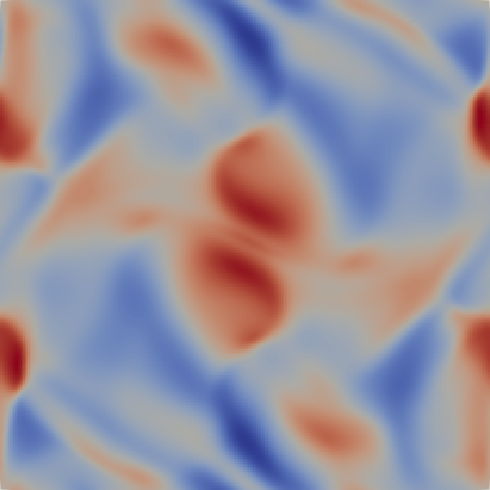
\includegraphics[width=\textwidth]{results/orszag_tang5}
  \end{subfigure}
  \caption{Density of the Orszag-Tang vortex (\autoref{sec:orszagtang}) at
    $t=0.5$ (top left), $t=2.0$ (top right), $t=3.0$ (bottom left) and $t=5.0$
    (bottom right).}
  \label{fig:orszagtang}
\end{figure}

\clearpage
\bibliographystyle{abbrv}
\bibliography{report}
\end{document}